\section{ROS} \label{sec:ros}
El sistema operativo para robots, conocido como ROS (Robot Operating System), se basa en una arquitectura de software distribuida que permite a los diferentes componentes de un robot —como sensores, actuadores y módulos de procesamiento— comunicarse de manera eficiente y flexible. La imagen presentada ilustra de forma clara cómo se lleva a cabo esta comunicación dentro de ROS, mediante el uso de nodos, temas y servicios.

\begin{figure}[h]
	\centering
	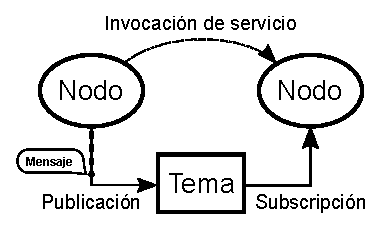
\includegraphics[width=0.5\linewidth]{img/ROS_concepts}
	\caption{Diagrama de comunicación de ROS}
	\label{fig:rosconcepts}
\end{figure}


\subsection{Nodo (Node)}
En el contexto de ROS (Robot Operating System), un nodo es una unidad fundamental de ejecución. Es, básicamente, un proceso independiente que se encarga de realizar una función específica dentro del sistema robótico. Un nodo puede ejecutar una tarea simple, como leer un sensor o mover una articulación, o tareas más complejas como realizar cálculos de trayectoria, procesar imágenes o tomar decisiones autónomas.
Un nodo como componente modular es una de las grandes ventajas de ROS es su arquitectura modular. Esta modularidad se logra dividiendo el sistema robótico en múltiples nodos, donde cada uno realiza una función única y especializada. Gracias a esto, el desarrollo de software se vuelve más organizado y flexible. Si un nodo falla o necesita mejoras, puede modificarse o reiniciarse sin afectar directamente a los demás nodos. Por ejemplo.

\begin{itemize}
    \item Un nodo de sensores puede estar constantemente leyendo datos de un sensor ultrasónico o una cámara.
    \item Un nodo de control puede estar calculando las señales necesarias para mover un motor basado en esos datos.
    \item Un nodo de navegación puede estar trazando rutas o evitando obstáculos.
\end{itemize}

\begin{figure}[h]
	\centering
	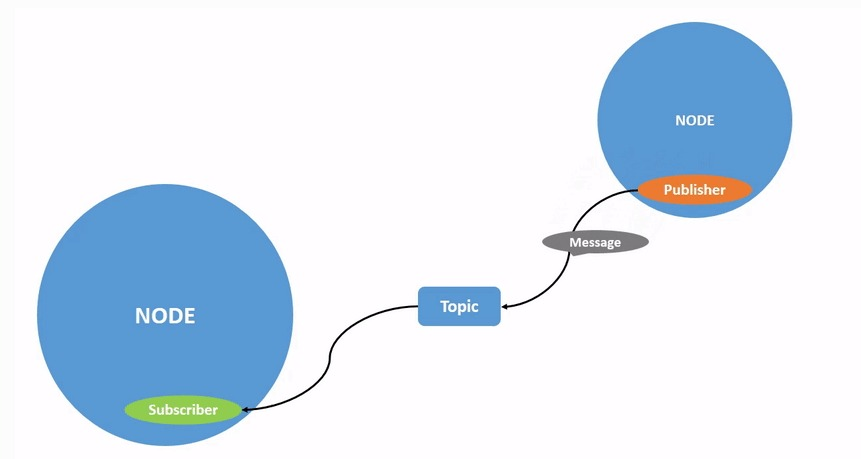
\includegraphics[width=0.5\linewidth]{img/NODOS ROS.jpeg}
	\caption{Nodos de ROS}
	\label{fig:NODOS ROS}
\end{figure}

En el entorno de ROS (Robot Operating System), la comunicación entre los distintos procesos que ejecutan tareas en un sistema robótico se establece a través de nodos, los cuales interactúan entre sí mediante un mecanismo de publicación y suscripción sobre un canal común denominado tópico. Cada nodo representa una unidad funcional autónoma que puede actuar como publicador (publisher), suscriptor (subscriber), o ambos.

En este esquema, un nodo publicador se encarga de generar información —como lecturas de sensores, comandos de movimiento, datos de estado, entre otros— y enviarla a un tópico específico. Dicha información es encapsulada en estructuras denominadas mensajes, que se transmiten de forma asíncrona. Por su parte, cualquier nodo que necesite esta información puede suscribirse al mismo tópico, recibiendo automáticamente los mensajes enviados por el publicador.

Esta arquitectura desacoplada permite que múltiples nodos puedan recibir datos de un solo publicador sin que exista una conexión directa entre ellos, fomentando así la modularidad, escalabilidad y flexibilidad del sistema. Además, esta relación facilita la implementación de sistemas distribuidos, ya que los nodos pueden ejecutarse en distintas máquinas mientras se comunican a través de los mismos tópicos.

\subsection{Tema (Topic)}
En ROS (Robot Operating System), un tópico es un canal de comunicación que permite la transmisión de datos entre nodos de manera asíncrona. Funciona como un "espacio común" donde los nodos publican y suscriben mensajes. Es uno de los mecanismos más usados en ROS para el intercambio de información en tiempo real, debido a su simplicidad, eficiencia y escalabilidad.


\textbf{Comunicacion basada en "topics"}

El sistema de comunicación por tópicos sigue un modelo publicador/suscriptor:
\begin{itemize}
    \item Un nodo que publica datos (por ejemplo, las lecturas de un sensor) lo hace hacia un tópico específico.
    \item Otro nodo, que se suscribe a ese mismo tópico, recibe los datos sin necesidad de conocer directamente al publicador.
\end{itemize}


\subsection{Mensaje (Message)}
En ROS (Robot Operating System), un mensaje es la unidad básica de datos que se intercambia entre nodos a través de un tópico. Cada mensaje es una estructura de datos predefinida y organizada, que permite la comunicación entre procesos distribuidos en un sistema robótico.
Los mensajes permiten transmitir información específica como posiciones, velocidades, imágenes o datos de sensores entre los diferentes componentes del sistema, de manera estandarizada y eficiente.
Un mensaje en ROS se define a través de archivos .msg, que especifican sus campos y tipos de datos. Estos pueden ser:
\begin{itemize}
    \item \textbf{Tipos primitivos:} int32, float64, bool, string, etc.
    \item \textbf{Tipos compuestos:} Estructuras definidas por otros mensajes.
    \item \textbf{Arreglos o listas:} De tipo primitivo o compuesto
\end{itemize}

\subsection{Servicio (Service)}
\subsection{Gazebo}
\subsection{RViz}
